
\chapter{Towards Classifier Visualisation in 3D Source Space}
\chaptermark{Towards Classifier Visualisation in 3D Source Space}%
\label{chapter:visualisation}%


{\chaptermeta

\textbf{Krol, L. R.\textsuperscript{1}, Mousavi, M.\textsuperscript{2}, de Sa, V. R.\textsuperscript{3}, \& Zander, T. O.\textsuperscript{4}}

{\small
\textsuperscript{1}Biological Psychology and Neuroergonomics, Technische Universität Berlin, Berlin, Germany
\textsuperscript{2}Electrical and Computer Engineering, University of California San Diego, San Diego, USA
\textsuperscript{3}Cognitive Science, University of California San Diego, San Diego, USA
\textsuperscript{4}Zander Laboratories B.V., Amsterdam, the Netherlands

This is the postprint version of the manuscript published as follows:

Krol, L. R., Mousavi, M., de Sa, V. R., \& Zander, T. O. (2018). Towards Classifier Visualisation in 3D Source Space. In \emph{2018 IEEE International Conference on Systems, Man and Cybernetics (SMC)} (pp. 71–76). doi: 10.1109/SMC.2018.00022\nocite{krol2018classvis}

© 2018 IEEE. Reprinted, with permission, from Krol, L. R., Mousavi, M., de Sa, V. R., \& Zander, T. O., Towards Classifier Visualisation in 3D Source Space, October 2018.
\par}}


\abstract%
In the context of brain-computer interfacing, it is important to investigate what regions of the brain a classifier focuses on. For one, this will clarify to what extent the classifier relies on brain activity, as opposed to undesirable non-cortical signals. More generally, the practice is informative as it allows conclusions to be drawn about the cortical regions---and thus, cortical functions---that contribute to the effect under investigation. In this study, we start to investigate different methods to visualise the regions of interest of classifiers based on windowed means and on common spatial patterns. Specifically, we take individually reconstructed source spaces and transform the classifier filter weights into relevance weights indicating the relative contribution of each source to the classifier. This is visualised across participants in an average brain. By decomposing the classifier weights into separate sources and localising these in the brain, this method provides a tool to evaluate classifiers and test hypotheses.


\clearpage


\fancypagestyle{visualisation}{%
    \fancyhf{}
    \fancyhead[EC]{\textit{\leftmark}}
    \fancyhead[OC]{\textit{\rightmark}}
    \fancyfoot[C]{\thepage \\ \vspace{6.8mm} \colorbox{footerbg}{\parbox{\paperwidth-2\fboxsep}{\centering\parbox{0.75\paperwidth}{\centering\fontsize{9pt}{9pt}\selectfont\textcolor{footerfg}{This is the postprint version of published manuscript: Krol, L. R., Mousavi, M., de Sa, V. R., \& Zander, T. O. (2018). \\ Towards Classifier Visualisation in 3D Source Space. In \textit{2018 IEEE International Conference on Systems, Man and Cybernetics (SMC)} (pp. 71–76). © 2018 IEEE.}}}}}
    \fancyfootoffset[]{1.25in}}
\pagestyle{visualisation}


\section{Introduction}

A brain-computer interface (BCI) allows an output channel to be established from a user's brain to a computer---an output channel ``that is neither neuromuscular nor hormonal'' \cite{wolpaw2012newsun}. Such a channel can be used in various ways. For example, it allows paralysed or locked-in patients to communicate with the outside world using mental spellers \cite{birbaumer1999spelling} and brain-actuated prostheses \cite{mullerputz2008ssvepprosthesis}. BCI-based systems enable people to control such and other devices using only their brain activity. 

A \emph{passive} brain-computer interface (pBCI) \cite{zander2011} is a BCI system that uses similar hard- and software in order to interpret ongoing, ``natural'' brain activity \cite{krol2018interactivity} that is not meant to control a device. Instead, such brain activity reflects the human user's cognitive or affective state. Passive BCI-based quantifications of mental states are used as \emph{implicit input} to support ongoing human-computer interaction \cite{zander2014implicit}. 

With recent trends in neuroadaptive technology and pBCI itself \cite{krol2017interactivitygraz,zander2017surgery,krol2016workload,zander2017phypa}, as well as advances in signal acquisition hardware \cite{zander2017dry}, such real-world pBCI applications have become increasingly close at hand. In particular, electroencephalography (EEG) has become increasingly mobile \cite{mullen2015dry}. An important issue with EEG however, is that many different sources of activity combine to form the final signal measured at the scalp. This includes not just numerous cortical sources, but all electromagnetic activity present in the body as well as in the environment. Notably, eye and muscle artefacts can contaminate the data.

During EEG experiments in realistic contexts, a great amount of eye and muscle activity is to be expected. Furthermore, this activity can be highly correlated to the experimental conditions. A classifier trained to distinguish between data reflecting different conditions can thus be highly influenced by such non-brain activity. Because of this, it is important to verify to what extent an advertised \emph{brain}-computer interface system is indeed based on \emph{brain} activity. For example, when a system is intended to measure negative affect from brain activity, it may inadvertently use activity from the corrugator muscle of the face \cite{larsen2003emgaffect}. Such a system may not be as reliable in different contexts (e.g. where sunshine leads to excessive squinting), and may be more accurately categorised as a form of physiological computing \cite{fairclough2009fundamentals}.

While detection of non-brain influences is one specific case where extended feature analysis can provide important answers, 
understanding the relative contributions of different brain sources is another.
A classifier is trained to distinguish between different conditions using any and all 
information available. This makes it a powerful method to distinguish between brain activity in different conditions \cite{noh2014dimred},
but also means that the classifier
can be influenced by a variety of cognitive processes.  
For example,
even when targeting a specific cognitive process such as motor imagery, activity from other processes may interfere with the recordings \cite{mousavi2017mi} and affect the classifier. 
Knowing what information carries what weight can help to validate the classifier and the experimental paradigm.  If the cortical areas that a classifier focuses on can be
identified, this may 
provide insights into the different cognitive processes underlying the investigated effects. 
When a classifier's primary source of distinguishing brain activity comes from the visual cortex, for example, this may hint that low-level sensory aspects of the stimuli were more important than further cognitive interpretation of those stimuli. 
Such insights can also be used to improve experimental paradigms and BCI training methods~\cite{mousavi2017training}.

In this paper we explore, with simulated data, aspects of a method used earlier \cite{zander2016nat} to visualise in a three-dimensional head volume the areas of the brain a BCI classifier focuses on. The original method applied only to windowed-means classifiers of event-related potentials \cite{blankertz2011}; here we describe an adaptation of that method, as well as an extension that applies to common spatial patterns \cite{ramoser2000}. 


\begin{figure*}[!t]
    \centering
    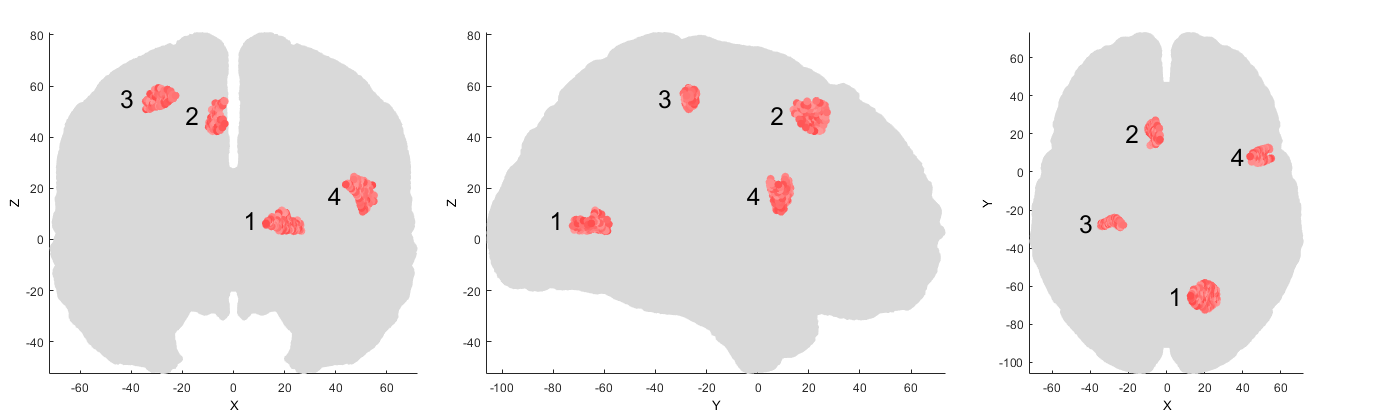
\includegraphics[width=0.989\textwidth]{figures/visualisation-groundtruth.png}
    \caption{Ground-truth locations in the brain of the simulated class-dependent signals, covering the 1.5~cm maximum deviation. In data set 1, source numbers 1 and 2 generated ERPs in one class, but not in the other. In data set 2, 1 and 2 generated alpha activity in one class, while 3 and 4 did so in the other.}
    \label{fig:visualisation:groundtruth}
\end{figure*}


\section{Methods}


\subsection{Data Simulation}

In order to have a known ground truth to evaluate the method, we used simulated EEG data. This was generated using SEREEGA \cite{krol2018sereega}, an open-source toolbox dedicated to simulating event-related EEG activity. Using the New York Head model and lead field \cite{huang2016nyhead}, two sets of 64-channel data were simulated. Each data set consisted of two conditions (classes) for the classifier to distinguish.

\paragraph{Data set 1} This data set contained systematic class differences in the temporal domain. One class consisted entirely of brown noise emanating from 64 sources spaced throughout the brain. The second class consisted of equally arranged noise, along with two event-related potentials (ERPs) emanating from two selected sources, respectively (numbered 1 and 2 in Figure~\ref{fig:visualisation:groundtruth}). The second source's ERP had an average amplitude four times greater than the other; however, this larger-amplitude ERP only occurred randomly in 25\% of epochs of that class. Single epoch amplitudes varied by 20\%. Both peaked at 300~ms $\pm$~50 with a width of 200~ms $\pm$~40.

\paragraph{Data set 2} This data set contained systematic class differences in the spectral domain. Both classes contained brown noise emanating from 64 sources spaced throughout the brain. Furthermore, each class contained additional uniform white noise filtered between 8 and 14~Hz, emanating from two sources each. In both classes, one source's signal amplitude was twice that of the other. (From Figure~\ref{fig:visualisation:groundtruth}, source numbers 1 and 2 were active in one class; 3 and 4 in the other.)

Note that the sources selected here do not reflect any deliberately chosen functional region. For the purposes of this paper, the selected regions' neuroscientific significance is not relevant: we merely wish to reconstruct their locations.

Each data set mentioned above consisted of 10 simulated `participants'. The non-noise brain source locations were relatively consistent across these participants, differing up to 1.5~cm across participants. (Note that a small shift in position can lead to a significant change in projection as, due to the cortical folds, the source will be oriented differently relative to the scalp.) The other sources were randomly distributed for each participant. A total of 100 epochs of 800~ms each were simulated for each class.

The signal-to-noise ratio was controlled in such a way that a cross-validated estimate of the classifier accuracy would roughly average 75--80\%, which are common rates for BCI applications.


\subsection{Classifier Visualisation in Putative Source Space}


\subsubsection{Separation of the Data into Sources}

We wish to visualise a classifier in putative source space. To that end, independent of any BCI classifier, the data must first be separated into putative sources. Different methods exist for this purpose. In this paper, we use independent component analysis (ICA) \cite{bell1995} as an example. ICA is a blind source separation method that decomposes the data $x$ into statistically maximally independent sources $s$ by finding a transformation or `unmixing' matrix $A$ such that $x=As$. $A$ is a filter matrix weighting the individual channel activations in sensor space to obtain the identified independent component activations. Inversely, $A^{-1}$ contains the forward model of these components, i.e., their projections onto the scalp. Other source separation methods will produce different contents of $A$, but their application in this method is essentially the same.

Independent EEG sources are dipolar \cite{delorme2012dipolar}. We can thus fit an equivalent dipole model to the forward ICA decomposition, e.g. using the EEGLAB toolbox DIPFIT 2.3 \cite{oostenveld2003dipfit}. The dipole model provides a 3D localisation for each independent component that minimises the residual variance between the dipole and the component projections.

For the results in this paper, since we used simulated data, we did not calculate $A$ on the data. Instead, we obtained the ground-truth mixing matrix directly from the simulation. The equivalent dipole model however was calculated separately using DIPFIT.


\subsubsection{Obtaining a Classifier}

The method presented here applies to linear discriminant analysis (LDA)-based spatio-temporal classifiers. In particular, we present results for common spatial patterns and the windowed-means approach.

In the windowed-means approach (WM) \cite{blankertz2011}, the mean amplitudes of the scalp activations at each electrode and in each time window are extracted as features, to which shrinkage LDA is applied to separate the classes. This results in LDA filter weights  $w_\textrm{WM}=\Sigma_\textrm{WM}^{-1}(\mu_{1}-\mu_{2})$ where $\mu_{1}$ and $\mu_{2}$ are the mean of the features for classes 1 and 2 respectively and $\Sigma_\textrm{WM}$ is the common class covariance.

Common spatial patterns (CSP) \cite{ramoser2000} are used to extract features in the frequency domain. CSP finds the optimal set of filter weights that maximise the variance of the filtered signal for one class while simultaneously minimising it for the other. Usually the top $m < \frac{C}{2}$ filters for each class are selected, where $C$ is the number of channels. The data in each epoch is spatially filtered to this new pseudo-channel space and the log of the signal's variance on each pseudo-channel is selected as the set of features for the classifier. We then apply a shrinkage LDA, resulting in LDA filter weights $w_\textrm{CSP}$. 


\subsubsection{Obtaining a Classifier's Forward Model}

In case of the WM classifier, the LDA filter weights cannot be neurophysiologically interpreted. As Haufe et al. explain, ``classifier weights can exhibit small amplitudes for measurement channels containing the signal-of-interest, but also large amplitudes at channels not containing this signal'' \cite{haufe2014}. Therefore, we must first transform the LDA filter weights into \emph{patterns}. For this paper, we did this by multiplying the LDA filter weights of the backward model by the regularised LDA's common covariance matrix (as opposed to the non-regularised version \cite{haufe2014}). Thus, the patterns $p_\textrm{WM}=\Sigma_\textrm{WM} w_\textrm{WM}=\mu_{1}-\mu_{2}$ show the differential scalp activity between classes.

For the CSP classifier, let CSP filters be columns of the matrix $W \in \mathbb{R}^{C\times C}$. CSP patterns are then defined to be columns of $P = (W^{-1})^T \in \mathbb{R}^{C\times C}$. Essentially, $P$ and $W$ are the forward and backward models, respectively. However, not each of the selected CSP filters contributes equally to classification. Their respective contributions depend on the LDA weights that were trained on their features. Here, the same LDA filter weight issues apply that were mentioned above. We thus transform these into interpretable weightings or forward weights indicating their relative contributions: $\tilde{w}_\textrm{CSP}=\Sigma_\textrm{CSP} w_\textrm{CSP}$ where $\Sigma_\textrm{CSP} \in \mathbb{R}^{2m \times 2m}$ is the common covariance of the CSP features from classes 1 and 2. We use these forward weights to scale the CSP patterns for visualisation: let $P_\textrm{sel} \in \mathbb{R}^{C\times 2m}$ be the CSP patterns corresponding to the $2m$ selected CSP filters, then the $i$-th column in $p_\textrm{CSP}$ is the $i$-th column in $P_\textrm{sel}$ scaled by the $i$-th element in $\tilde{w}_\textrm{CSP}$.  

We now have patterns representing the forward model for these classifiers in the form of weights for each electrode. For WM, we have one pattern for each time window. For CSP, we have $m$ weighted patterns for each class.


\subsubsection{Projecting the Classifier Patterns into Source Space}

The ICA's unmixing matrix $A^{-1}$ transforms sensor-level scalp activations into source activations. Similarly, it can transform sensor-level weights into corresponding weights in source space. When patterns contain class-relevant scalp projections, projecting these into source space gives us the \emph{relevance weights} $w_r=|A^{-1} p|$ that indicate how the different source activations linearly combine to create these patterns. In other words, the relevance weights reflect to what extent the sources contribute to the patterns. By extension, the relevance weights thus reflect to what extent the sources contribute to the class differences. For our purpose, the sign of the weights is not relevant at this point, hence we take the absolute value.

In case of WM, we now have one set of relevance weights per time window per participant. In case of CSP, we have  $2m$ sets per participant. Each set contains as many weights as we have independent components for that participant.


\subsubsection{Alternative Source Weights}
\label{visualisation:alternative}

Using different methods can give different perspectives on the data. We have explained how sensor-level patterns can be transformed to obtain source-level relevance weights. Alternatively, source-level weights can be calculated in source space directly, independent of the classifier. For example, we can use Pearson correlation to obtain a set of weights for the WM case.

To that end, we first repeat the feature extraction in source space, i.e., we obtain the mean of each source activation in each time window. We then calculate the correlation coefficient between these source features $F_s$ and the vector of true class labels $L$ to obtain a set of weights $w_\textrm{WMcorr} = |corr(F_s,L)|$. The sign is irrelevant for our purpose. 


\subsubsection{Visualising Relevance Weights in Source Space}

In case of WM, we generate one visualisation per time window, each illustrating the sources contributing to the class differences at that time. In case of CSP, we generate one per class, illustrating the sources distinctive for that class.

For each time window or class, respectively, the obtained relevance weights are distributed to the dipole locations of the corresponding sources for each participant. We then generate a weighted 3D kernel density plot containing these weights for all participants in one plot. For this, we use the EEGLAB plug-in dipoleDensity v0.36 \cite{miyakoshi2013dipdens} which aligns the output to slices of the mean MNI brain. For the figures in this paper, we used a smoothing kernel of 12~mm. 

\begin{figure*}[t]
    \centering
    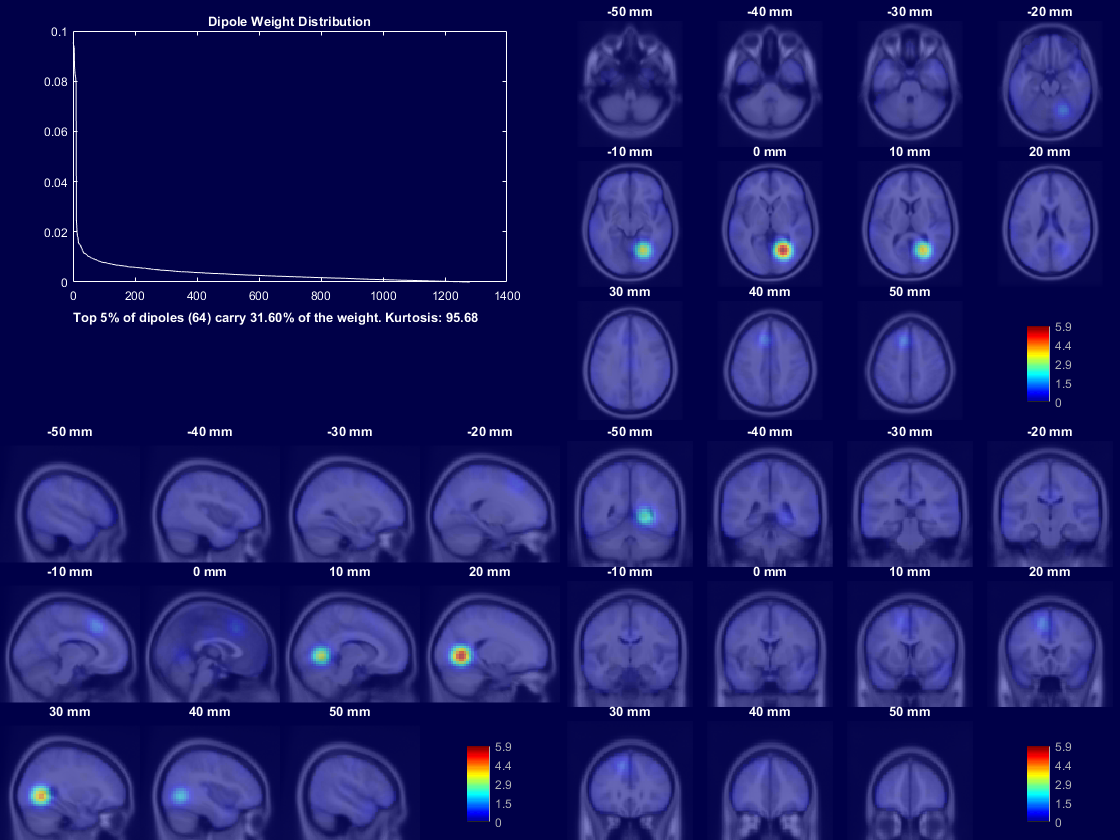
\includegraphics[width=\textwidth]{figures/visualisation-result_CSP_class2.png}
    \caption{Visualisation of the CSP classifier: class 1. Slices are labelled with their corresponding MNI coordinates. Top left: sorted dipole weight distribution.}
    \label{fig:visualisation:csp2}
\end{figure*}


\begin{figure}[t]
    \centering
    \subfloat[]{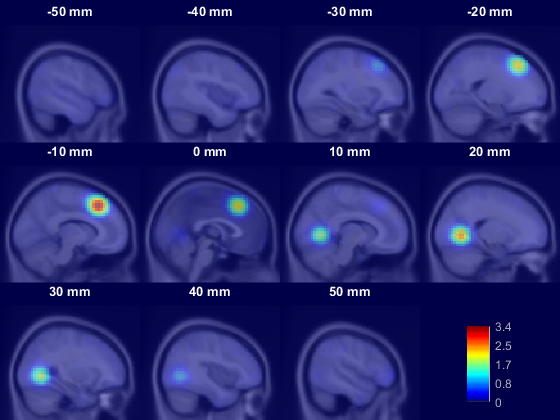
\includegraphics[width=0.45\textwidth]{figures/visualisation-result_ERP_LDA_sagittal.png}}%
    \qquad
    \subfloat[]{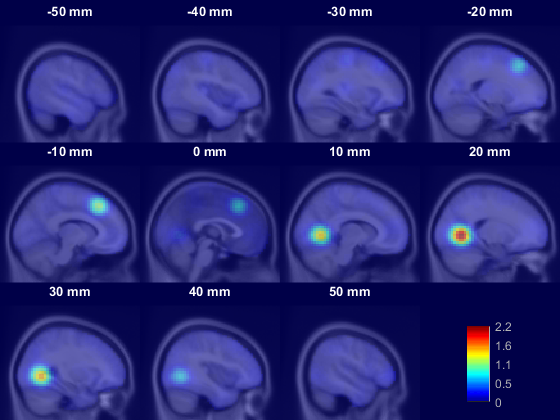
\includegraphics[width=0.45\textwidth]{figures/visualisation-result_ERP_correlation_sagittal.png}}%
    \caption{Left (a): Partial visualisation (sagittal section) of the WM classifier: projected LDA weights. Right (b): Partial visualisation (sagittal section) of source feature class correlation in data set 1: source correlation weights.}
    \label{fig:visualisation:erpldacorr}
\end{figure}

\begin{figure}[t]
    \centering
    \subfloat[]{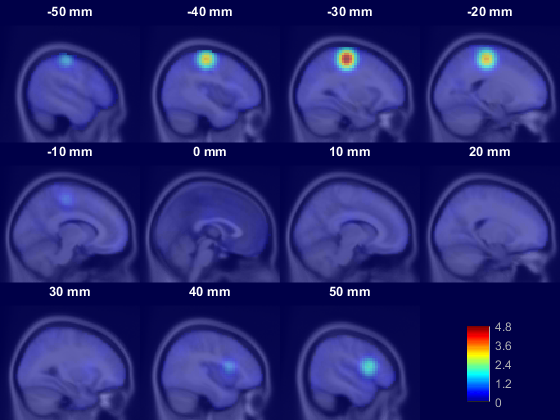
\includegraphics[width=0.45\textwidth]{figures/visualisation-result_CSP_class1_sagittal.png}}
    \qquad
    \subfloat[]{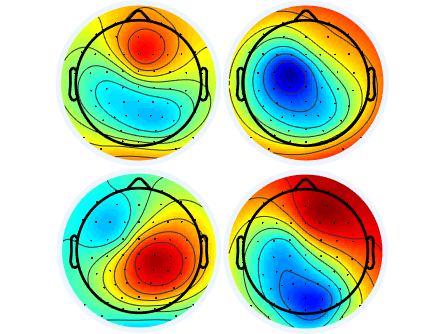
\includegraphics[width=0.45\textwidth]{figures/visualisation-erp_projections_2x2.png}}
    \caption{Left (a): Partial visualisation (sagittal section) of the CSP classifier: class 2. Right (b): Combined projection patterns of the two class-dependent sources in data set 1, for four of the simulated participants.}
    \label{fig:visualisation:csp1proj}
\end{figure}


\section{Results}

Figure~\ref{fig:visualisation:csp2} shows the output of the presented method for all participants in one case. The top left shows the sorted distribution of the relevance weights. The other panels show different slices of the mean MNI brain along with the colour-coded weighted dipole density, or `relevance density'. The sparse distribution indicates that a relatively small number of sources receive a relatively high percentage of weights. In other words, the method shows that the differences between the classes can be traced back to a relatively specific area in the brain.

Figure~\ref{fig:visualisation:csp2} visualises class 1 of the CSP classifier calibrated on data set 2. We see that the most dense, i.e. the most relevant area is near source number 1 in figure~\ref{fig:visualisation:groundtruth}. A second, weaker area of relevance is near source number 2. This accurately reflects the simulation of data set 2, where class 1 was defined by activity in these two sources, with the signal amplitude of source number 1 twice that of source number 2.

To preserve space, the other figures only show the sagittal density slices. Figure~\ref{fig:visualisation:csp1proj} (left) visualises the second class of data set 2, as identified by the CSP classifier. This accurately reflects the correct locations of source numbers 3 and 4.

Figure~\ref{fig:visualisation:erpldacorr} (left) visualises the regions of interest of the LDA classifier calibrated on data set 1 in a selected time window. This, too, accurately reflects the ground truth that sources in the right-occipital and left-frontal lobes (i.e. numbers 1 and 2 in figure~\ref{fig:visualisation:groundtruth}) were generators of the class differences. Notably, we see that the sources are weighted roughly equally, with source 2 weighted only slightly more than source 1. This is in line with the signals that were generated by these two sources. The amplitude of source 2 was four times that of source 1. However, the probability of a signal occurring at all in source 2 was only 25\%, whereas source 1 was active in each simulated trial. The mean amplitude of these sources over all trials was thus roughly the same, but their predictive value was not.

Figure~\ref{fig:visualisation:erpldacorr} (right) visualises the alternative weights for data set 1, described in section~\ref{visualisation:alternative}. We see a high correlation density for source number 1 and a significantly lower density for source number 2. This reflects the difference in predictive value between sources 1 and 2.


\section{Summary}

We simulated two data sets of 10 simulated participants each. Each participant's data was simulated with unique locations for the generator sources, with some consistency maintained for the sources that generated the class differences. In one data set, these class differences were caused by the presence of event-related potentials from two sources. In the other, differences were caused by the presence of alpha-band activity in different sources. An ICA solution was available for the simulated data.

Two different classifiers were trained on the two data sets respectively: A WM classifier, focusing on temporal differences between the classes in data set 1, and a CSP classifier, focusing on spectral differences in data set 2.

For the WM classifier, we transformed the LDA filter weights into patterns representing the forward model. For the CSP classifier, we separated the produced CSP patterns and weighted them by computed forward weights.

We then transformed these patterns into relevance weights connected to independent components using the unmixing matrix of each participant's data's ICA solution. Since a 3D position in the brain was calculated for each of these independent components, we were able to generate a `relevance density plot' indicating the classifiers' regions of interest. As we used simulated EEG data, we compared the obtained results to the known ground truth and could verify that the generated plots corresponded to the original sources.  

For the WM classifier, we also presented an alternative method to calculate relevance weights directly in source space. This method can provide a different perspective on the brain dynamics underlying the class differences.


\section{Discussion}

In our earlier work \cite{zander2016nat} we presented a combination of the two WM-based methods discussed here, where the classifier's regions of interest were additionally weighted by those regions' class-correlation. In this paper we simulated data that highlights how these two methods can provide different perspectives when used separately.

The use of simulated data enabled us to compare the method's results to a known ground truth. We see that under these circumstances, the method accurately recovers the correct sources in the brain. Of course, simulated data represents only a first test case. The previous iteration of this method has already been shown to produce results in line with hypotheses on real EEG data \cite{zander2016nat}, and we will continue this work by validating the current method on other real EEG recordings. We will also extend the method to filter-bank CSP \cite{ang2008fbcsp}, and make all code available for free.

Simulated data also allowed us to use a ground-truth ICA decomposition to initially control for the varying results that different ICA methods provide. In future work, we will furthermore apply the method to simulated data with ICA decompositions of varying quality. And, since estimating the covariance matrix is a fundamental step in producing the patterns, we will further investigate the influence of different covariance estimation methods on the patterns and their projections into source space.

The method presented here visualises the areas in the brain that the classifier focuses on, for two popular classification methods. The patterns that can be obtained from these classifiers can be neurophysiologically interpreted on their own \cite{haufe2014}. However, the current method provides two additional advantages. First of all, the patterns are decomposed into individual sources. A single pattern can consist of the combined projections of any number of different sources, and different source projections can interfere with each other to the point of making interpretation difficult. For example, figure~\ref{fig:visualisation:csp1proj} (right) shows the combined projection patterns of the two class-dependent sources in data set 1 for four of the simulated participants. As we can see, minor changes in source location and orientation produce large differences in the projection pattern. From these patterns, it is not obvious that they are produced by two distinct sources, let alone their location. With accurate ICA models, we can untangle this relation and show individual source contributions to the classifier. 

Secondly, this method uses an equivalent dipole model to visualise the sources in 3D space. Projection patterns coming from roughly the same cortical area can vary markedly between participants due to anatomical differences. A 3D visualisation of the cortical areas corrects for these differences in a way that e.g. a mean projection pattern cannot. We visualise the combined relevance weights of all participants in a single plot to highlight the most consistently relevant areas.

It is important to be able to perform an inspection of a classifier's regions of interest, and compare the results to our hypotheses as well as other perspectives on the data. When we design a BCI application, we hypothesise what functions (and thus, what regions) of the brain will be targeted. Visualisation methods such as this one enable us to compare a classifier's actual regions of interest to these hypotheses, and validate our assumptions---and to gather new insights about the cortical processes underlying the observed effects.


\section*{Acknowledgements}

This work was supported by the Deutsche Forschungsgemeinschaft (ZA 821/3-1), a Short-Term Research Grant awarded to MM by the German Academic Exchange Service, and the National Science Foundation (IIS 1528214).


\section*{References}

A shared bibliography starts at page~\pageref{bibliography}.


\clearpage
\pagestyle{plain}
